\\
\textbf{Integrationstests}\\
Integrationstestene som gruppen har fokuseret på, er tests af API ‘ets primære funktionalitet. 
Hertil nogle simple tests af hvilket dataformat der returneres og hvilken HTTP kode som returneres. 
Størstedelen af de test som bliver eksekveret i dette projekt, er test af API ‘ets ”Get Request”, men 
”AuthController’en” bliver testet med nogle ”Post” kald. \\

Optimalt ville en test database blive opsat som en kopi af den orginale og det ville være denne som 
blev testet og ikke den ”rigtige” database. Her skulle det ikke tages højde for hvilket data blev indsat 
eller nødvendigvis at fjerne det igen.\\ 

\textbf{Testing Framework}\\
Beskrevet i indledningen er testing et fundament for et hvert udviklings team, til at sikre 
kvalitet og funktionalitet af koden. Efter undersøgelse af mulighederne i ”dotnet” besluttede 
gruppen at anvende frameworket NUnit hertil. \\

NUnit er et framework til alle ”dotnet” sprog og er uddraget fra JUnit som anvendes til Java, 
hvilket gruppen arbejdede med i sidste semester projekt.\\

\textbf{TestCases}\\
Projektets 28 test udføres ved hjælp af datasæt som oprettes i en folder ”TestData” i projektet 
”NordicBio.NUnitTest”. Folderen indeholder centralt data og specifikke datasæt til hver controller 
som bliver testet. \\

\begin{figure}[!h]
    \centering
    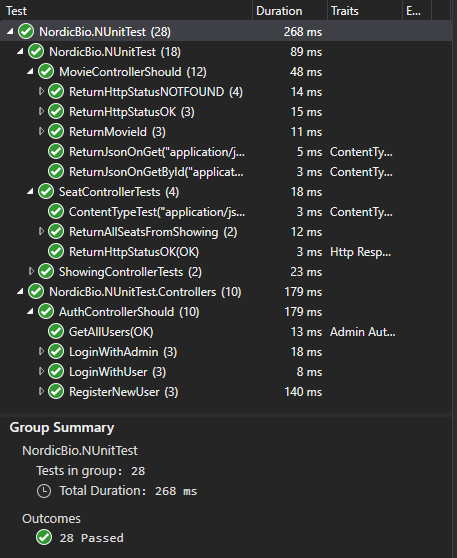
\includegraphics[width=0.8\textwidth]{figures/testpassing.PNG}
    \caption{Tests Passing}
    \label{fig:testpassing}
\end{figure}

I hver klasse findes metoder som returnerer forskellige datasæt én efter én ved hjælp af nøgleordet 
”yield return”. Datasættet er specificeret ved hjælp af klassen ”TestCaseData” som tager de parametre 
som skal testes og de bliver efterfølgende parset ind i metoden som parametre i den rækkefølge de er sat.\\

Denne tilgang sikre få metoder og hurtig tilførsel af nye datasæt uden af fjerne eller tilføje nye metoder. 
Det nye datasæt skal blot tilføjes til klassen og den metode som er tilknyttet.\\

Hver test følger denne logik og anvender ”Arrange, Act og Assert” til strukturering af testene. 



